% Provenance (never printed): see sources/outline_sources.md (Year 2: Hadean, Archean and
% Proterozoic; early crust and greenstone belts; the oxygenation of the atmosphere; snowball
% Earth). Eons and eras from the ICS chart; greenstone belts, TTG and cratons after Cawood and
% others (2018) and Smithies and others (2019); komatiite liquidus after Sossi and O'Neill (2016),
% Pierru and others (2022) and Asimow (2022); the Archean air and the GOE after Catling and Zahnle
% (2020) and Luo and others (2016); the boring billion after Lyons and others (2021); snowball
% Earth after Hoffman and others (2017). The energy-balance model, the komatiite line and the CO2
% build-up from figdata/bachelor-2/precambrian.py; exercise and problem values in the Book 4
% scratch calculator calc/ch18.py.
\chapter{प्रीकैम्ब्रियन पृथ्वी}\label{ch:b2:precambrian-earth}

पहले कवचधारी जीवाश्म लगभग 540 मिलियन वर्ष पुरानी चट्टानों में दिखते हैं। उनसे पहले का सब कुछ,
\qty{4567}{Ma} पहले पृथ्वी के जन्म से, प्रीकैम्ब्रियन है: ग्रह के इतिहास का सात-आठवाँ भाग।
उस समय में पृथ्वी ने अपने महाद्वीपों के क्रोड बनाए, अपनी वायु को ऑक्सीजन से भरा,
और कम से कम दो बार ध्रुवों से भूमध्य रेखा तक जम गई, जब हिमचादरें उष्णकटिबंध में समुद्र तक
पहुँचीं। यह अध्याय उन चार अरब वर्षों को उनसे बची चट्टानों में पढ़ता है,
और उनकी तीन पहेलियों को संख्याओं में रखता है: सबसे पुराने लावा इतने गर्म क्यों थे, जमा हुआ
ग्रह कैसे पिघल सकता है, और युवा पृथ्वी मंद सूर्य के नीचे गर्म कैसे रही।
% ledger: ics:base.Hadean, ics:base.Phanerozoic, hoffman17:cryochrons

\begin{recall}
\textbf{स्कूल की पुस्तकों से}: पृथ्वी की आयु; भूवैज्ञानिक समय-मापक्रम पर महाकल्प;
युवा सूर्य की दीप्ति का नियम और \omterm{def:b2:precambrian-earth:faint-sun}{मंद युवा सूर्य की समस्या}; आदिम वायुमंडल;
स्ट्रोमैटोलाइट, पट्टित लौह संरचनाएँ, \omterm{def:b2:precambrian-earth:goe}{महा ऑक्सीकरण घटना} और लाल संस्तर; \omterm{def:b2:precambrian-earth:craton}{क्रेटॉन};
अतीत में रेडियोजनिक ऊष्मा। \textbf{पुस्तक 3 (स्नातक वर्ष 1) से}: ज़िरकॉन और उसकी U--Pb आयु,
अवरोध-तापमान; चार समस्थानिकों का रेडियोजनिक ऊष्मा-उत्पादन; बाह्य दीर्घ-तरंग
विकिरण और वैश्विक माध्य सूर्यातप $S_0/4$; कालस्तरिक इकाइयाँ।
\textbf{पिछले अध्यायों से}: \omterm{def:b2:mantle-melting:tp}{प्रावार का विभव तापमान} और रुद्धोष्म
(\cref{ch:b2:mantle-melting}); ओलिवीन का लिक्विडस और प्रभाजी क्रिस्टलन
(\cref{ch:b2:magmatic-differentiation}); ग्रेनाइट के प्रकार (\cref{ch:b2:crustal-melting});
\omterm{def:b2:wilson-cycle:supercontinent}{महामहाद्वीप} (\cref{ch:b2:wilson-cycle})। ऑक्सीकरण और अपचयन रसायन की
पुस्तकों के विषय हैं, और पहले यूकैरियोट और प्रकाश-संश्लेषण जीवविज्ञान की पुस्तकों के।
\end{recall}

\section{जीवाश्मों से पहले के तीन महाकल्प}\label{sec:b2:precambrian-earth:eons}

\begin{definition}[हेडियन, आर्कियन, प्रोटेरोज़ोइक]\label{def:b2:precambrian-earth:eons}
फ़ैनेरोज़ोइक से पहले का समय तीन महाकल्पों में बँटा है। \emph{हेडियन}\index{हेडियन}
पृथ्वी के बनने, \qty{4567}{Ma} पहले, से $4031 \pm \qty{3}{Ma}$ तक चलता है;
\emph{आर्कियन}\index{आर्कियन} $4031$ से \qty{2500}{Ma} तक;
\emph{प्रोटेरोज़ोइक}\index{प्रोटेरोज़ोइक} 2500 से \qty{538.8}{Ma} तक, यानी कैम्ब्रियन के आधार तक।
मिलकर उन्हें अनौपचारिक रूप से प्रीकैम्ब्रियन कहा जाता है।
\end{definition}
% ledger: ics:base.Hadean, ics:base.Archean, ics:base.Proterozoic, ics:base.Phanerozoic

\omterm{def:b2:precambrian-earth:eons}{आर्कियन} चार महायुगों में बँटा है, इओआर्कियन (4031 से \qty{3600}{Ma}), पैलियोआर्कियन (3600
से 3200), मेसोआर्कियन (3200 से 2800) और नियोआर्कियन (2800 से 2500); \omterm{def:b2:precambrian-earth:eons}{प्रोटेरोज़ोइक} तीन में,
पैलियोप्रोटेरोज़ोइक (2500 से \qty{1600}{Ma}), मेसोप्रोटेरोज़ोइक (1600 से 1000) और
नियोप्रोटेरोज़ोइक (1000 से 538.8)। आगे दो नियोप्रोटेरोज़ोइक काल महत्त्वपूर्ण हैं, क्रायोजेनियन, 720 से
\qty{635}{Ma}, और एडियाकरन, 635 से \qty{538.8}{Ma}।
% ledger: ics4:archean-eras, ics4:proterozoic-eras

\begin{omfigure}
\centering
% ledger: ics:base.Hadean, ics:base.Archean, ics:base.Proterozoic, ics:base.Phanerozoic, ics4:archean-eras, ics4:proterozoic-eras, wilde01:4404, bowring99:acasta, cz20:impacts, allwood06:spc, cawood18:transition, gumsley17:goe, luo16:goe, hoffman17:earlier, earle:bif, lyons21:boring, hoffman17:ages, asimow22:komatiite
\begin{tikzpicture}[x=-3.4cm, y=1cm, font=\scriptsize]
% eons
\fill[icsHadean] (4.567,0) rectangle (4.031,0.5);
\fill[icsArchean] (4.031,0) rectangle (2.5,0.5);
\fill[icsProterozoic] (2.5,0) rectangle (0.5388,0.5);
\fill[icsPhanerozoic] (0.5388,0) rectangle (0,0.5);
\node[text=white] at (4.299,0.25) {हेडियन};
\node[text=white] at (3.27,0.25) {आर्कियन};
\node[text=white] at (1.52,0.25) {प्रोटेरोज़ोइक};
\node at (0.27,0.25) {फ़ैने॰};
% eras
\foreach \a/\b/\c in {4.031/3.6/35, 3.6/3.2/55, 3.2/2.8/35, 2.8/2.5/55}
  \fill[icsArchean!\c] (\a,-0.45) rectangle (\b,0);
\foreach \a/\b/\c in {2.5/1.6/35, 1.6/1.0/55, 1.0/0.5388/35}
  \fill[icsProterozoic!\c] (\a,-0.45) rectangle (\b,0);
\foreach \x/\l in {3.8155/इओ, 3.4/पैलियो, 3.0/मेसो, 2.65/नियो, 2.05/पैलियो, 1.3/मेसो, 0.769/नियो}
  \node at (\x,-0.225) {\l};
% axis
\draw (4.6,-0.6) -- (0,-0.6);
\foreach \t in {0,0.5,...,4.5} {
  \draw (\t,-0.6) -- (\t,-0.7);
  \node[anchor=north] at (\t,-0.7) {\pgfmathprintnumber[fixed, precision=1]{\t}};
}
\node[anchor=north, font=\small] at (2.3,-1.05) {वर्तमान से पहले का समय (अरब वर्ष)};
% row A
\fill[omDef] (4.404,0.85) circle (2pt);
\node[anchor=west, text=omDef] at (4.404,0.85) {सबसे पुराना ज़िरकॉन};
\fill[omMeth] (3.43,0.85) circle (2pt);
\node[anchor=west, text=omMeth] at (3.43,0.85) {पहले स्ट्रोमैटोलाइट};
\draw[red!60!black, line width=3pt] (2.4,0.85) -- (1.8,0.85);
\node[anchor=west, text=red!60!black] at (1.8,0.85) {पट्टित लौह संरचनाएँ};
% row B
\fill[omDef] (4.03,1.5) circle (2pt);
\node[anchor=west, text=omDef] at (4.03,1.5) {सबसे पुरानी चट्टानें};
\draw[black!70, line width=3pt] (3.2,1.5) -- (2.5,1.5);
\node[anchor=south, text=black!80] at (2.85,1.6) {विवर्तनिक शैली में परिवर्तन};
\draw[omProp, line width=3pt] (1.8,1.5) -- (0.8,1.5);
\node[anchor=south, text=omProp] at (1.3,1.6) {``नीरस अरब वर्ष''};
% row C
\draw[black!60, line width=2pt, densely dashed] (4.2,2.25) -- (3.5,2.25);
\node[anchor=south, text=black!70] at (3.85,2.35) {विलंबित भारी बमबारी? (विवादित)};
\draw[omThm, line width=3pt] (2.43,2.25) -- (2.06,2.25);
\node[anchor=west, text=omThm] at (2.06,2.25) {महा ऑक्सीकरण घटना};
% row D
\fill[blue!60!black] (2.4,3.0) circle (2pt);
\node[anchor=east, text=blue!60!black] at (2.4,3.0) {पहली हिमगोल पृथ्वी};
\fill[omThm] (0.8,3.0) circle (2pt);
\node[anchor=east, text=omThm] at (0.8,3.0) {ऑक्सीजन की दूसरी वृद्धि};
% row E
\fill[orange!80!black] (1.9,3.7) circle (2pt);
\node[anchor=east, text=orange!80!black] at (1.9,3.7) {अंतिम सामान्य कोमैटिआइट};
\draw[blue!60!black, line width=3pt] (0.717,3.7) -- (0.635,3.7);
\node[anchor=east, text=blue!60!black] at (0.717,3.7) {क्रायोजेनियन हिमगोल पृथ्वियाँ};
% row F
\fill[omMeth] (0.57,4.4) circle (2pt);
\node[anchor=east, text=omMeth] at (0.57,4.4) {पहले बड़े जीवाश्म (एडियाकरन)};
\end{tikzpicture}
\par\smallskip{\small एक रेखा पर प्रीकैम्ब्रियन। महाकल्प और, हल्के रंगों में, उनके महायुग
(इओ-, पैलियो-, मेसो- और नियोआर्कियन; पैलियो-, मेसो- और नियोप्रोटेरोज़ोइक) अंतरराष्ट्रीय
कालस्तरिक चार्ट के हैं; घटनाएँ पाठ में उद्धृत आयु पर रखी गई हैं।
``अंतिम सामान्य \omterm{def:b2:precambrian-earth:greenstone}{कोमैटिआइट}'' ऐलुमिनियम-अनवक्षीण प्रकार के हैं; नए, दुर्लभतर प्रकार भी मिलते हैं।}
\end{omfigure}

\subsection*{हेडियन: चट्टानों के बिना खनिज}

\omterm{def:b2:precambrian-earth:eons}{हेडियन} से कोई चट्टान नहीं बची, केवल खनिज। सबसे पुराना पश्चिमी ऑस्ट्रेलिया की जैक
हिल्स का ज़िरकॉन का एक कण है, $4404 \pm \qty{8}{Myr}$ पुराना, जो किसी पुरानी चट्टान से बहकर निकला और
कोई तीन अरब वर्ष पहले एक संगुटिकाश्म में जमा हुआ। उसके और उसके पड़ोसी कणों के संघटन को
उसके खोजकर्ताओं ने इस बात का प्रमाण माना कि महाद्वीपीय प्रकार की भूपर्पटी और
तरल जल \qty{4.4}{Gyr} पहले ही मौजूद थे, पृथ्वी बनने के कोई 160 मिलियन वर्ष बाद।
सबसे पुरानी तिथि-निर्धारित चट्टानें, उत्तर-पश्चिमी कनाडा की अकास्टा नाइस, 4.00 से
\qty{4.03}{Ga} पुरानी हैं, \omterm{def:b2:precambrian-earth:eons}{आर्कियन} के आधार के निकट।
% ledger: wilde01:4404, wilde01:zircon, uw14:jack-hills, bowring99:acasta

युवा पृथ्वी पर बड़े पिंड टकराए, जैसा \cref{ch:b2:planet-formation-meteorites}
ने वर्णन किया। पूरे महासागर को वाष्पित करने लायक बड़ा अंतिम संघट्ट
लगभग \qty{4.3}{Ga} पहले हुआ माना जाता है। बाद की एक ``विलंबित भारी
बमबारी'', लगभग 4.2--4.0 और \qty{3.5}{Ga} के बीच संघट्टों की एक बौछार, जो
चंद्र चट्टानों और उल्कापिंडों में आघातों की आयु से अनुमानित है, प्रस्तावित की गई है; बहुत से विवाद करते हैं कि वह
कोई अलग घटना थी भी, और किसी भी स्थिति में उसने शायद पृथ्वी को निर्जीव नहीं किया होगा।
% ledger: cz20:impacts

\section{आर्कियन भूपर्पटी}\label{sec:b2:precambrian-earth:archean}

\subsection*{हरितप्रस्तर पट्टियाँ और कोमैटिआइट}

बची हुई \omterm{def:b2:precambrian-earth:eons}{आर्कियन} भूपर्पटी दो प्रकार के भूभागों से बनी है, अगल-बगल: धूसर,
सोडियम-समृद्ध ग्रेनाइटी नाइस के बड़े पिंड, और परिवर्तित ज्वालामुखीय और अवसादी चट्टान की सँकरी पट्टियाँ।

\begin{definition}[हरितप्रस्तर पट्टी; कोमैटिआइट]\label{def:b2:precambrian-earth:greenstone}
\emph{हरितप्रस्तर पट्टी}\index{हरितप्रस्तर पट्टी} मैफ़िक और अल्ट्रामैफ़िक ज्वालामुखीय चट्टानों की एक पट्टी है,
अवसादों सहित, जो निम्न श्रेणी पर कायांतरित हैं (हरा रंग क्लोराइट, ऐक्टिनोलाइट और
एपिडोट से आता है), और \omterm{def:b2:precambrian-earth:eons}{आर्कियन} और कुछ \omterm{def:b2:precambrian-earth:eons}{प्रोटेरोज़ोइक} भूभागों में ग्रेनाइटॉइड के पिंडों के बीच स्थित है।
\emph{कोमैटिआइट}\index{कोमैटिआइट} एक अल्ट्रामैफ़िक लावा है, बेसाल्ट से कहीं अधिक MgO-समृद्ध,
जो द्रव के रूप में उद्गारित हुआ; उसका ओलिवीन प्रायः लंबे, पतले फलकों में उगता है, यानी
\emph{स्पिनिफ़ेक्स} बनावट, जब प्रवाह का शीर्ष तेज़ी से ठंडा होता है।
\end{definition}
% ledger: cawood18:dome-keel, so16:liquidus, pierru22:komatiite

\begin{omfigure}
\centering
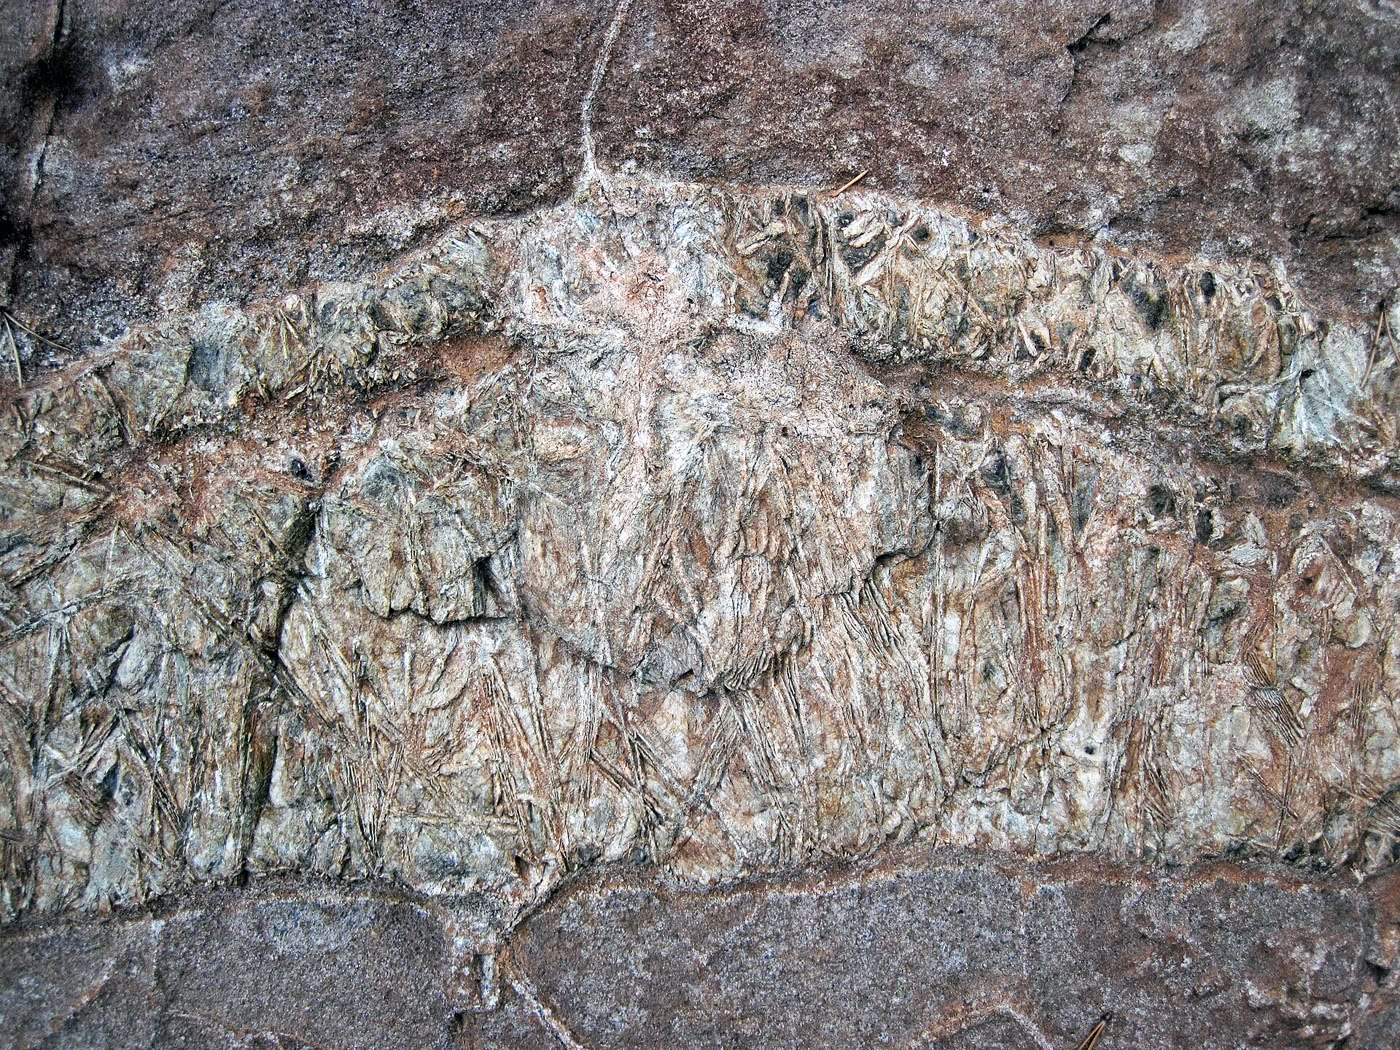
\includegraphics[width=0.66\linewidth]{images/book4/b2-18-spinifex-komatiite.jpg}
\par\smallskip{\small एक \omterm{def:b2:precambrian-earth:greenstone}{कोमैटिआइट} प्रवाह में स्पिनिफ़ेक्स बनावट, पाइक हिल, ओंटारियो, लगभग 2.71 अरब वर्ष पुरानी
एक नियोआर्कियन \omterm{def:b2:precambrian-earth:greenstone}{हरितप्रस्तर पट्टी} का भाग: ओलिवीन के फलक, अब परिवर्तित,
प्रवाह के ठंडे होते शीर्ष के आर-पार उगे। फ़ोटो: James St.~John, CC~BY~2.0 (Wikimedia
Commons)।}
\end{omfigure}

\omterm{def:b2:precambrian-earth:greenstone}{कोमैटिआइटों} में \qty{34}{\percent} तक MgO होता है, जबकि आज के कटकों के प्राथमिक
बेसाल्टों में 10 से \qty{13}{\percent}, और वे लगभग पुरानी पृथ्वी तक सीमित हैं: ऐलुमिनियम-क्षीण
प्रकार केवल \qty{2.8}{Ga} से पुरानी चट्टानों में मिलता है, ऐलुमिनियम-अनवक्षीण प्रकार लगभग
\qty{1.9}{Ga} तक, और केवल एक दुर्लभ ऐलुमिनियम-समृद्ध प्रकार \qty{90}{Myr} जितना नया है। मैग्नीशियम में
इतना समृद्ध गलित बहुत गर्म होता है, और,
\cref{ch:b2:magmatic-differentiation} के बेसाल्टों की तरह, उससे क्रिस्टलित होने वाला पहला खनिज ओलिवीन है,
जिसका द्रव में अंश तापमान को तय करता है।
% ledger: pierru22:komatiite, asimow22:komatiite

\begin{proposition}[कोमैटिआइट तापमापी]\label{prop:b2:precambrian-earth:liquidus}
वायुमंडलीय दाब पर ओलिवीन के साथ साम्य में किसी गलित का लिक्विडस तापमान
गलित की MgO मात्रा के साथ लगभग रैखिक रूप से बढ़ता है। दो प्रयोगों $(m_1, T_1)$ और
$(m_2, T_2)$ से होकर,
\[
  T_{\text{लिक्विडस}}(m) = T_1 + s\,(m - m_1), \qquad s = \frac{T_1 - T_2}{m_1 - m_2} .
\]
दो \omterm{def:b2:precambrian-earth:greenstone}{कोमैटिआइटों} पर गलन-प्रयोग, $\qty{32.2}{\percent}$ MgO \qty{1616}{\celsius} पर और
$\qty{23}{\percent}$ \qty{1450}{\celsius} पर, $s = \qty{18.0}{\celsius}$ प्रति प्रतिशत
MgO देते हैं।
\end{proposition}
% ledger: so16:liquidus, helz98:glass-thermometer

\begin{proof}
ओलिवीन फ़ॉर्स्टेराइट और फ़ेयालाइट का एक ठोस विलयन है, जिस गलित से वह उगता है उससे मैग्नीशियम में
कहीं अधिक समृद्ध। जैसे-जैसे गलित ठंडा होता है, ओलिवीन उससे मैग्नीशियम निकालता है, और वह तापमान
जिस पर गलित ओलिवीन में ठीक संतृप्त होता है, उसकी MgO मात्रा के साथ गिरता है। प्रयोग दिखाते हैं कि
गलितों के किसी दिए गए परिवार के परास पर यह गिरावट लगभग रैखिक है, अतः
दो प्रयोगों से होकर जाने वाली रेखा उनके बीच अंतर्वेशन करती है; $s = (1616 - 1450)/(32.2 - 23) = 166/9.2 = 18.04$।
\end{proof}

यह गुणांक \omterm{def:b2:precambrian-earth:greenstone}{कोमैटिआइटों} के लिए विशेष नहीं है। किलाउआ के लावा से द्रुत-शीतित काँच,
उसी तरह अंशांकित, \qty{3}{\celsius} बदलते हैं, \qty{0.15}{\percent} MgO के लिए, यानी
प्रति प्रतिशत \qty{20}{\celsius}। \omterm{def:b2:precambrian-earth:greenstone}{कोमैटिआइट} रेखा को \qty{12}{\percent} MgO वाले
किसी प्राथमिक कटक-बेसाल्ट तक नीचे बढ़ाने पर उसका लिक्विडस कुछ दसियों डिग्री के भीतर मिलता है: $1616 -
18.0\times20.2 \approx \qty{1252}{\celsius}$। अतः सबसे गर्म \omterm{def:b2:precambrian-earth:greenstone}{कोमैटिआइट} द्रव
आज के कटकों को पोषित करने वाले गलितों से कोई \qty{360}{\celsius} अधिक गर्म थे, और नीचे का चित्र
रेखा दिखाता है।
% ledger: helz98:glass-thermometer, so16:liquidus, pierru22:komatiite
% values: slope 18.043, T_morb12 1251.5, dT_kom_morb 364.5 (precambrian.py)

\begin{omfigure}
\centering
\begin{tikzpicture}
\begin{axis}[omrecord, width=0.72\linewidth, height=6cm, xmin=8, xmax=35, ymin=1150, ymax=1700,
  xlabel={गलित में MgO (द्रव्यमान से \unit{\percent})}, ylabel={1 atm पर लिक्विडस (\unit{\celsius})},
  xtick pos=bottom, ytick pos=left, clip=false,
  y tick label style={/pgf/number format/1000 sep={}}]
% computed in figdata/bachelor-2/precambrian.py part kom; ledger: so16:liquidus, pierru22:komatiite
\fill[omProp!15] (axis cs:10,1150) rectangle (axis cs:13,1700);
\addplot[black, line width=1.1pt] table[x=MgO, y=T] {figdata/out/bachelor-2-precambrian-kom.dat};
\addplot[only marks, mark=*, mark size=2.4pt, omThm] coordinates {(32.2,1616) (23,1450)};
\node[anchor=north west, font=\scriptsize, text=omThm] at (axis cs:32.2,1612) {बारबर्टन};
\node[anchor=north west, font=\scriptsize, text=omThm] at (axis cs:23,1446) {मुनरो};
\node[anchor=south, font=\scriptsize, text=omProp, align=center] at (axis cs:11.5,1560)
  {प्राथमिक\\कटक-बेसाल्ट};
\draw[densely dashed] (axis cs:12,1150) -- (axis cs:12,1251.5) -- (axis cs:8,1251.5);
\draw[densely dashed] (axis cs:32.2,1150) -- (axis cs:32.2,1616);
\draw[<->, omDef, thick] (axis cs:27,1251.5) -- (axis cs:27,1616);
\draw[densely dotted] (axis cs:12,1251.5) -- (axis cs:27,1251.5);
\draw[densely dotted] (axis cs:27,1616) -- (axis cs:32.2,1616);
\node[anchor=east, font=\scriptsize, text=omDef] at (axis cs:26.7,1330) {लगभग \qty{360}{\celsius}};
\end{axis}
\end{tikzpicture}
\par\smallskip{\small \omterm{def:b2:precambrian-earth:greenstone}{कोमैटिआइट} तापमापी: दो \omterm{def:b2:precambrian-earth:greenstone}{कोमैटिआइटों} (बिंदु) पर मापे गए लिक्विडस तापमानों से होकर
जाने वाली रेखा, आज के कटकों के प्राथमिक बेसाल्टों के 10 से \qty{13}{\percent} MgO (पट्टी) तक
बढ़ाई गई। यह विस्तार बेसाल्टी गलितों के मिलते-जुलते ढाल पर टिका है।}
\end{omfigure}

अधिक गर्म लावा का अर्थ उतनी ही मात्रा में अधिक गर्म प्रावार नहीं है। \omterm{def:b2:precambrian-earth:greenstone}{कोमैटिआइट} शायद
प्रावार-स्तंभों में उठे, जैसे आज के सबसे गर्म बेसाल्ट हवाई में उठते हैं, जहाँ विभव तापमान
लगभग \qty{200}{\celsius} तक ऊपर है, परिवेशी प्रावार के $1350 \pm \qty{50}{\celsius}$ से। और
वे गलन की बड़ी मात्राओं से, अधिक गहराई पर, बने। सामान्यतः माना जाता है कि वे
आज के प्रावार से 200 से \qty{300}{K} गर्म प्रावार में बने; एक वैकल्पिक मत के अनुसार
\omterm{def:b2:precambrian-earth:greenstone}{कोमैटिआइट} जलयुक्त \omterm{def:b2:magma-emplacement:magma}{मैग्मा} थे, जो आसपास के प्रावार से बहुत अधिक नहीं, ऐसे तापमानों पर बने।
किसी भी स्थिति में, \omterm{def:b2:precambrian-earth:eons}{आर्कियन} प्रावार अधिक गर्म था, और स्कूल की
पुस्तकों ने एक कारण दिया: 3 अरब वर्ष पहले चार रेडियोधर्मी समस्थानिक आज की ऊष्मा के दुगुने से अधिक
मुक्त करते थे (\cref{exo:b2:precambrian-earth:2})।
% ledger: asimow22:komatiite, pierru22:komatiite, so16:liquidus

\subsection*{TTG और गुंबद-और-कील प्रतिरूप}

\omterm{def:b2:precambrian-earth:greenstone}{हरितप्रस्तर पट्टियों} के बीच की धूसर नाइस उस प्रकार के ग्रेनाइट नहीं हैं जिनका
\cref{ch:b2:crustal-melting} ने वर्णन किया।

\begin{definition}[टोनालाइट--ट्रॉन्डजेमाइट--ग्रैनोडायोराइट समूह]\label{def:b2:precambrian-earth:ttg}
\emph{टोनालाइट--ट्रॉन्डजेमाइट--ग्रैनोडायोराइट समूह}\index{टोनालाइट--ट्रॉन्डजेमाइट--ग्रैनोडायोराइट समूह}
(TTG) सोडियम-समृद्ध, पोटैशियम-निर्धन ग्रेनाइटॉइडों का परिवार है --- टोनालाइट,
ट्रॉन्डजेमाइट (मैफ़िक खनिजों में निर्धन टोनालाइट) और ग्रैनोडायोराइट --- जो
\omterm{def:b2:precambrian-earth:eons}{आर्कियन} महाद्वीपीय भूपर्पटी का अधिकांश भाग बनाता है। उनमें से अधिकांश जलयोजित बेसाल्टी
भूपर्पटी के \omterm{def:b2:mantle-melting:melting}{आंशिक गलन} से बने।
\end{definition}
% ledger: smithies19:ttg, cawood18:ttg

आज की महाद्वीपीय भूपर्पटी के आयतन का बड़ा भाग \omterm{def:b2:precambrian-earth:eons}{आर्कियन} के अंत तक बन चुका था, अधिकांशतः
TTG के रूप में। कुछ TTG में सूक्ष्म-तत्व चिह्न हैं जिन्हें लंबे समय तक
\qty{50}{km} से अधिक गहराई पर गलन माना गया, ऐसा दाब जो नई महाद्वीपीय भूपर्पटी में नहीं पहुँचता, और ये व्याख्याएँ
इस बहस में भार रखती हैं कि प्लेट विवर्तनिकी कब शुरू हुई; 2019 के एक अध्ययन ने तर्क दिया कि वे चिह्न
इसके बजाय प्रावार के गलितों से आते हैं, और कि सामान्य TTG
किसी आज की सामान्य महाद्वीपीय भूपर्पटी के \qty{40}{km} से अधिक नहीं, ऐसी गहराइयों पर बने। \omterm{def:b2:precambrian-earth:eons}{आर्कियन} के अंत में,
लगभग 3.0 और \qty{2.5}{Ga} के बीच, अधिकांश \omterm{def:b2:precambrian-earth:craton}{क्रेटॉनों} के ग्रेनाइटॉइड TTG से
पोटैशियम-समृद्ध ग्रेनाइटों में बदल जाते हैं, जो किसी मोटी भूपर्पटी के फिर से गलने का संकेत है।
% ledger: smithies19:ttg, cawood18:ttg

ऑस्ट्रेलिया के पूर्वी पिलबारा में, ज़िम्बाब्वे में और दक्षिणी भारत में, दोनों भूभाग मानचित्र पर एक
प्रभावशाली प्रतिरूप बनाते हैं। ग्रेनाइटॉइड के गोल गुंबद हरितप्रस्तर की अभिनत कीलों से घिरे हैं जिनकी परतें गुंबदों से दूर की ओर नत और अभिमुख हैं। गुंबदों के बारे में
माना जाता है कि वे \omterm{def:b2:magma-emplacement:ascent}{डायापिरों} के रूप में उठे, हल्की ग्रेनाइटी भूपर्पटी लावाओं के एक मोटे, सघन ढेर के आर-पार
उठी जो उनके बीच धँसा। पिलबारा में यह गुंबदन सैकड़ों मिलियन
वर्षों तक चला और लगभग \qty{3.1}{Ga} पहले रुका, जिसके बाद संरचनाएँ रैखिक हो जाती हैं, जैसे
नए पर्वतजनों की।
% ledger: cawood18:dome-keel

\begin{omfigure}
\centering
\begin{tikzpicture}[x=0.95cm, y=0.95cm, font=\scriptsize]
% schematic, after the description in cawood18:dome-keel
\fill[lith basalt] (0,0) rectangle (12,7);
\draw (0,0) rectangle (12,7);
\foreach \cx/\cy/\rx/\ry in {2.4/4.7/1.7/1.4, 7.2/5.0/2.0/1.4, 4.6/1.6/1.9/1.1, 10.0/2.0/1.4/1.3}
  \filldraw[lith granite, draw=black, thick] (\cx,\cy) ellipse ({\rx} and {\ry});
% strike and dip in the greenstone, each dipping away from the nearest dome
% (positions and strikes from the outward normals of the ellipses, computed by hand)
\foreach \px/\py/\st in {3.9/5.99/309, 0.9/5.99/231, 0.9/3.41/129, 2.4/2.88/90, 4.52/4.7/0,
    9.62/5.0/0, 8.91/6.29/305, 5.49/6.29/235, 8.91/3.71/55, 5.49/3.71/125,
    6.92/1.6/0, 4.6/3.12/270, 2.28/1.6/180, 6.24/0.53/60,
    10.0/3.72/270, 11.29/0.78/47, 8.18/2.0/180, 11.29/3.22/313}
  \pic at (\px,\py) {strikedip={\st}{}};
\node[fill=white, inner sep=1.5pt] at (2.4,4.7) {TTG गुंबद};
\node[fill=white, inner sep=1.5pt] at (7.2,5.0) {TTG गुंबद};
\node[fill=white, inner sep=1.5pt] at (4.6,1.6) {TTG गुंबद};
\node[fill=white, inner sep=1.5pt] at (10.0,2.0) {TTG गुंबद};
\node[fill=white, inner sep=1.5pt, align=center] at (7.45,2.75) {हरितप्रस्तर\\कील};
\node[fill=white, inner sep=1.5pt, align=center] at (1.0,0.9) {हरितप्रस्तर};
\pic at (11.4,5.6) {northarrow};
% section below
\begin{scope}[yshift=-3.3cm]
\fill[lith basalt] (0,0) -- (12,0) -- (12,2.2) -- (0,2.2) -- cycle;
\filldraw[lith granite, draw=black, thick] (0.6,0) .. controls (0.6,2.0) and (4.6,2.0) .. (4.6,0) -- cycle;
\filldraw[lith granite, draw=black, thick] (6.4,0) .. controls (6.4,2.1) and (11.0,2.1) .. (11.0,0) -- cycle;
\draw[thick] (0,0) rectangle (12,2.2);
\draw[black!70] (4.6,0.9) .. controls (5.5,0.2) .. (6.4,0.9);
\draw[black!70] (4.35,1.5) .. controls (5.5,0.6) .. (6.65,1.5);
\node[fill=white, inner sep=1.5pt] at (2.6,0.6) {TTG};
\node[fill=white, inner sep=1.5pt] at (8.7,0.6) {TTG};
\node[fill=white, inner sep=1.5pt] at (5.5,1.75) {कील};
\draw[->, thick] (2.6,1.0) -- (2.6,1.75);
\draw[->, thick] (8.7,1.05) -- (8.7,1.8);
\draw[->, thick] (5.5,1.4) -- (5.5,0.95);
\node[anchor=west] at (12.1,1.1) {काट};
\end{scope}
\node[anchor=west] at (12.1,3.5) {मानचित्र};
\end{tikzpicture}
\par\smallskip{\small कुछ \omterm{def:b2:precambrian-earth:eons}{आर्कियन} \omterm{def:b2:precambrian-earth:craton}{क्रेटॉनों} का गुंबद-और-कील प्रतिरूप (योजनामूलक, पैमाने के
बिना)। मानचित्र: हरितप्रस्तर से घिरे TTG समूह के ग्रेनाइटॉइड गुंबद; नति-और-दिक्स्थिति
चिह्न हरितप्रस्तरों की परतों को हर गुंबद से दूर नत होते दिखाते हैं। काट: गुंबद
उठते हैं जबकि सघन हरितप्रस्तर ढेर उनके बीच की अभिनत कीलों में धँसता है (तीर)।}
\end{omfigure}

\subsection*{क्रेटॉन}

\begin{definition}[क्रेटॉन]\label{def:b2:precambrian-earth:craton}
\emph{क्रेटॉन}\index{क्रेटॉन} किसी महाद्वीप का वह भाग है जो एक अरब वर्ष से अधिक
विवर्तनिक रूप से स्थिर रहा है: \omterm{def:b2:precambrian-earth:eons}{आर्कियन} या \omterm{def:b2:precambrian-earth:eons}{प्रोटेरोज़ोइक} भूपर्पटी का, कायांतरित और
पातालीय, एक क्रोड, जो स्थलमंडलीय प्रावार की एक मोटी, ठंडी और उत्प्लावक जड़ पर टिका है जो कोई
\qty{250}{km} गहराई तक पहुँचती है।
\end{definition}
% ledger: tulane:cratons, fischer:lithosphere, cawood18:ttg

\omterm{def:b2:precambrian-earth:craton}{क्रेटॉन} अधिकांशतः मेसोआर्कियन और नियोआर्कियन में स्थिर हुए, और उनकी
स्थिरता के चिह्न चट्टानों में लिखे हैं: उन पर बिछी चौड़ी अवसादी द्रोणियाँ, जैसे
कापवाल \omterm{def:b2:precambrian-earth:craton}{क्रेटॉन} पर ट्रांसवाल महासमूह (लगभग 2640 से \qty{2055}{Ma}) और पिलबारा पर माउंट ब्रूस
महासमूह (2775 से \qty{2210}{Ma}); सीधी \omterm{def:b2:magma-emplacement:bodies}{डाइकों} के झुंड जो उन्हें
भंगुर प्लेटों की तरह काटते हैं; और उनकी मोटी जड़ें, जो \omterm{def:b2:precambrian-earth:eons}{आर्कियन} के अंत तक बन चुकी थीं। 3.2 और
\qty{2.5}{Ga} के बीच अभिलेख सबसे पुराने निष्क्रिय किनारे और \omterm{def:b2:alpine-orogen:foreland}{अग्रभूमि द्रोणियाँ}, युग्मित
\omterm{def:b2:metamorphic-facies:metamorphism}{कायांतरण} की पट्टियाँ, और यह पुराचुंबकीय प्रमाण भी दिखाता है कि \omterm{def:b2:precambrian-earth:craton}{क्रेटॉन} एक-दूसरे के सापेक्ष खिसके।
2018 की एक समीक्षा इन परिवर्तनों को आज जैसी काम करती प्लेट विवर्तनिकी के क्रमिक आरंभ के रूप में पढ़ती है,
साथ ही ज़ोर देती है कि कोई अकेला प्रेक्षण इसे सिद्ध नहीं करता; उस आरंभ के प्रकाशित अनुमान
\omterm{def:b2:precambrian-earth:eons}{हेडियन} से नियोप्रोटेरोज़ोइक तक फैले हैं।
% ledger: cawood18:transition, cawood18:ttg, cawood18:cratons

\begin{inthefield}[हरितप्रस्तर पट्टी को पढ़ना]
किसी \omterm{def:b2:precambrian-earth:greenstone}{हरितप्रस्तर पट्टी} में मानचित्रण करने वाले भूवैज्ञानिक का पहला प्रश्न यह होता है कि चट्टानों के बनते समय
ऊपर किस ओर था, क्योंकि परतें प्रायः ऊर्ध्वाधर या उलटी होती हैं। तकिया-लावा
अपने गोल शीर्षों और उन नुकीले आधारों से उत्तर देते हैं जिन्हें वे नीचे के तकियों में धँसाते हैं; क्रमित परतें
ऊपर की ओर अपने महीन होने से; और \omterm{def:b2:precambrian-earth:greenstone}{कोमैटिआइट} प्रवाह अपने मंडलन से, एक द्रुत-शीतित और विभंगित शीर्ष
जिसमें स्पिनिफ़ेक्स फलक नीचे की ओर उगते हैं, ढेर हुए ओलिवीन क्रिस्टलों से समृद्ध आधार के ऊपर। स्टेशन-दर-स्टेशन
मानचित्रित अभिमुखता-दिशाएँ कीलों के अभिनतियों को खींचती हैं। फ़ेल्सिक टफ़ों
और गुंबदों के TTG से ज़िरकॉन फिर U--Pb आयु देते हैं, ताकि भूवैज्ञानिक बता सके कि कौन-से
हरितप्रस्तर उन गुंबदों से पुराने हैं जो अब उन्हें धकेलकर पार करते हैं।
\end{inthefield}
% ledger: so16:liquidus (spinifex in the top zones of flows), cawood18:dome-keel

\section{ऑक्सीजन}\label{sec:b2:precambrian-earth:oxygen}

\subsection*{ऑक्सीजन के बिना आर्कियन वायु}

स्कूल की पुस्तकों का आदिम वायुमंडल नाइट्रोजन और कार्बन डाइऑक्साइड में समृद्ध और
ऑक्सीजन में निर्धन था। प्रॉक्सी और प्रतिरूप अब उसे अधिक कसकर सीमित करते हैं। \qty{2.4}{Ga} से पहले सतह पर ऑक्सीजन
आज की मात्रा के दस लाखवें भाग से कम थी; कार्बन डाइऑक्साइड शायद आज की 10 से 2500
गुना और मीथेन 100 से \num{10000} गुना। यूरेनिनाइट और पाइराइट के कण, जिन्हें
ऑक्सीजन नष्ट करती है, \omterm{def:b2:precambrian-earth:eons}{आर्कियन} नदियों द्वारा ढोए गए और अपरिवर्तित जमा हुए; \qty{2.415}{Ga} पर
अपरदी यूरेनिनाइट का बचे रहना ऑक्सीजन को \qty{3.2e-5}{atm} तक सीमित करता है। कार्बन चक्र, जिसे
नीचे याद किया गया है, माध्य सतह-तापमान को लगभग 0 और \qty{40}{\celsius} के बीच रखता था।
% ledger: cz20:archean-air, kasting25:indicators

ऑक्सीजन बन रही थी: साइनोबैक्टीरिया प्रकाश-संश्लेषण से उसे मुक्त करते हैं, और कुछ \omterm{def:b2:precambrian-earth:eons}{आर्कियन} चट्टानों में
उसके हल्के निशान दिखते हैं। पर वह बनते ही खप जाती थी, ज्वालामुखीय गैसों द्वारा और समुद्र में घुले
लोहे द्वारा।
% ledger: luo16:goe, lyons21:boring

\begin{definition}[पट्टित लौह संरचना]\label{def:b2:precambrian-earth:bif}
\emph{पट्टित लौह संरचना}\index{पट्टित लौह संरचना}
(BIF) लौह ऑक्साइडों --- हेमेटाइट, मैग्नेटाइट --- और
चर्ट की पतली एकांतर परतों का एक रासायनिक अवसाद है। यह घुले लौह(II) वाले समुद्री जल से
अवक्षेपित होती है, जब वह लोहा अघुलनशील लौह(III) में ऑक्सीकृत होता है; अतः इसके लिए ऑक्सीजन-रहित
गहरा महासागर, लोहे की आपूर्ति, और जहाँ लोहा जमा होता है वहाँ एक ऑक्सीकारक चाहिए।
\end{definition}
% ledger: earle:bif, holland06:stages

पट्टित लौह संरचनाएँ 2.4 से \qty{1.8}{Ga} तक सबसे प्रचुर हैं; उसके बाद गहरे महासागर में
पर्याप्त घुला लोहा नहीं रहा, और वे लगभग लुप्त हो जाती हैं, क्रायोजेनियन के हिमनदीय निक्षेपों में
थोड़े समय के लिए लौटने के लिए (नीचे)। वे लोहे का एक सामान्य अयस्क हैं
(\cref{ch:b2:ore-deposits})।
% ledger: earle:bif, hoffman17:models

\subsection*{महा ऑक्सीकरण घटना}

\begin{definition}[महा ऑक्सीकरण घटना]\label{def:b2:precambrian-earth:goe}
\emph{महा ऑक्सीकरण घटना}\index{महा ऑक्सीकरण घटना} (GOE) वह अंतराल है, लगभग
2.4--2.3 से लगभग \qty{2.1}{Ga} तक, जिसके दौरान ऑक्सीजन पहली बार स्थायी रूप से वायुमंडल
और उथले महासागर में संचित हुई, अपनी वर्तमान मात्रा के दस लाखवें भाग से कम से बढ़कर
शायद दसवें भाग तक।
\end{definition}
% ledger: cz20:goe, cz20:archean-air, gumsley17:goe, holland06:stages

सबसे स्पष्ट चिह्नक सल्फ़र समस्थानिकों का एक हस्ताक्षर है। GOE से पुराने अवसादों में
सल्फ़र के समस्थानिक इस तरह छँटे हैं जैसा केवल ऑक्सीजन-रहित वायु में प्रकाश-रसायन
उत्पन्न करता है; ऑक्सीजन आने पर यह हस्ताक्षर गायब हो जाता है। इसकी भौतिकी और इसका पूरा अभिलेख
पुस्तक 5 का विषय हैं; यहाँ यह एक घड़ी का काम करता है। दक्षिण अफ़्रीका के ट्रांसवाल
महासमूह के आर-पार तीन वेधन-कोरों में यह हस्ताक्षर \qty{2.33}{Ga} पर, 1 से \qty{10}{Myr} के भीतर, गायब होता है:
वृद्धि स्वयं तेज़ थी। अन्य अभिलेख घटना का आरंभ 2.46 से \qty{2.43}{Ga} पर रखते हैं,
पहले वैश्विक हिमनदन के समय, और दिखाते हैं कि उसके बाद ऑक्सीजन
लगातार नहीं बढ़ी।
% ledger: luo16:goe, farquhar00:sulfur, pk02:anoxic, gumsley17:goe

GOE के बाद लाल संस्तर दिखते हैं, अपरदी पाइराइट और यूरेनिनाइट नदी की रेत से गायब हो जाते हैं,
और मृदाएँ अपना लोहा ऑक्साइडों के रूप में रखती हैं। पर गहरा महासागर एक अरब से अधिक
वर्षों तक अनॉक्सी रहा।
% ledger: kasting25:indicators, lyons21:boring

\subsection*{``नीरस अरब वर्ष'' और दूसरी वृद्धि}

लगभग 1.8 से \qty{0.8}{Ga} तक का अंतराल समुद्री कार्बोनेटों के कार्बन समस्थानिकों में इतना कम परिवर्तन दिखाता है
कि उसे व्यापक रूप से ``नीरस अरब वर्ष'' कहा जाता है। उसकी ऑक्सीजन विवादित है: आरंभिक
अनुमानों ने वर्तमान मात्रा का 1 से \qty{40}{\percent} दिया, क्रोमियम समस्थानिक
\qty{1}{\percent} से कम, शायद \qty{0.1}{\percent}, सुझाते हैं। गहरा महासागर अनॉक्सी था। इस अंतराल में
यूकैरियोट, जैसा जीवविज्ञान की पुस्तकें बताती हैं, प्रकट हुए, विविधीकृत हुए और संख्या में बढ़े। लगभग \qty{800}{Ma} से बहुत से अभिलेख
ऑक्सीजन की एक दूसरी, अचानक वृद्धि दिखाते हैं, जटिल जीवन के बड़े विकासों के समय; क्या
ऑक्सीजन ने उन्हें प्रेरित किया या उनके पीछे आई, इस पर अब भी बहस है। एडियाकरन के बड़े जीवाश्म
लगभग \qty{570}{Ma} से दिखते हैं। इस बीच \cref{ch:b2:wilson-cycle} के \omterm{def:b2:wilson-cycle:supercontinent}{महामहाद्वीप}
जुड़े और टूटे: निष्क्रिय किनारे, जो विखंडन का चिह्न हैं, लगभग 2100 से
\qty{1850}{Ma} के आसपास प्रचुर हैं, जब नूना जुड़ा, और फिर 650 से \qty{500}{Ma} तक।
% ledger: lyons21:boring, lyons21:eukaryotes, cawood18:ttg, nance22:supercontinents

\section{भूमध्य रेखा तक बर्फ़}\label{sec:b2:precambrian-earth:snowball}

\subsection*{हिम--एल्बिडो प्रतिपुष्टि}

हिम और बर्फ़ अपने पर पड़ने वाले सूर्य-प्रकाश का अधिकांश भाग परावर्तित करते हैं, खुला समुद्र बहुत कम: महासागर के लिए लगभग
\qty{6}{\percent}, नंगी समुद्री बर्फ़ के लिए 50 से \qty{70}{\percent}, हिम से ढकी बर्फ़ के लिए
\qty{90}{\percent} तक। ठंडी होती पृथ्वी अधिक बर्फ़ बनाती है, अधिक
सूर्य-प्रकाश परावर्तित करती है और और भी ठंडी होती है।
% ledger: nsidc:albedo-ice, albedo:surfaces

\begin{definition}[हिम--एल्बिडो प्रतिपुष्टि]\label{def:b2:precambrian-earth:ice-albedo}
\emph{हिम--एल्बिडो प्रतिपुष्टि}\index{हिम--एल्बिडो प्रतिपुष्टि} तापमान के किसी परिवर्तन का उस हिम और बर्फ़ के आवरण के परिवर्तन द्वारा
प्रवर्धन है जो वह उत्पन्न करता है: शीतलन बर्फ़ को फैलाता है, जो
ग्रह का एल्बिडो बढ़ाती है, अवशोषित सूर्य-प्रकाश घटाती है और ग्रह को और ठंडा करती है;
तापन उलटी दिशा में काम करता है। यह एक धनात्मक प्रतिपुष्टि है।
\end{definition}
% ledger: hoffman17:hysteresis, nsidc:albedo-ice

इसके परिणाम सबसे सरल जलवायु प्रतिरूप में दिखते हैं: एक तापमान $T$ और प्रति वर्ग मीटर ऊष्मा-धारिता
$C$ वाला एक ग्रह। वह $\tfrac14 S(1 - a)$ अवशोषित करता है, जहाँ $S$ उसकी दूरी पर सूर्य-प्रकाश
है और $a$ उसका एल्बिडो, और वह पुस्तक 3 का बाह्य दीर्घ-तरंग विकिरण खोता है,
जिसे $\varepsilon\sigma T^4$ लिखा जाता है: $\varepsilon$, यानी \emph{प्रभावी उत्सर्जकता},
मापती है कि सतह के उत्सर्जन का कितना भाग ग्रीनहाउस से बच निकलता है, और आज वह
$240.2/(\sigma\times288^4) = 0.616$ है। प्रतिपुष्टि को सम्मिलित करने के लिए एल्बिडो को
तापमान का फलन बनाया जाता है। यह अध्याय $a = 0.294$, आज का मान, लेता है जब $T \ge \qty{283}{K}$; $a
= 0.6$, वह मान जो जलवायु प्रतिरूप किसी वैश्विक रूप से जमी सतह को देते हैं, जब $T \le \qty{263}{K}$; और
बीच में एक सीधी रेखा। दोनों देहलियाँ एक प्रतिरूपण-चयन हैं, मापी गई
राशियाँ नहीं।
% ledger: earth:TSI, earth:albedo, earth:Tsurf, const:sigma, hoffman17:models
% values: eps 0.6158 (precambrian.py)

\begin{proposition}[ऊर्जा-संतुलन प्रतिरूप के साम्य]\label{prop:b2:precambrian-earth:ebm}
प्रतिरूप
\[
  C\,\frac{\mathrm dT}{\mathrm dt} = \tfrac14 S\bigl(1 - a(T)\bigr) - \varepsilon\sigma T^4
  = R(T) - E(T),
\]
में स्थिर तापमान $R(T) = E(T)$ के हल हैं। कोई स्थिर तापमान $T^*$
स्थायी है यदि $E'(T^*) > R'(T^*)$ और अस्थायी यदि $E'(T^*) < R'(T^*)$।
\end{proposition}

\begin{proof}
$R = E$ के किसी हल पर दायाँ पक्ष शून्य हो जाता है, अतः $T$ वहीं रहता है। उसके निकट, $T = T^*
+ \delta$ रखिए: प्रथम कोटि तक $C\,\dot\delta = (R'(T^*) - E'(T^*))\,\delta$, जिसका हल
$\delta(t) = \delta(0)\,e^{(R' - E')t/C}$ क्षयित होता है जब $E' > R'$ और बढ़ता है जब $E' < R'$।
\end{proof}

$E$ हमेशा $T$ के साथ बढ़ता है। $R$ वहाँ सपाट है जहाँ एल्बिडो नियत है, अतः जमा हुआ और गर्म
साम्य स्थायी हैं; उनके बीच के ढलान में $R$ बढ़ता है, क्योंकि तापन बर्फ़ पिघलाता है, और यदि वह
$E$ से तेज़ बढ़ता है तो वहाँ का साम्य अस्थायी है। नीचे का चित्र दिखाता है कि आज के
सूर्य-प्रकाश के साथ प्रतिरूप के तीन साम्य हैं।

\begin{example}[आज के सूर्य के नीचे तीन जलवायु]\label{ex:b2:precambrian-earth:three}
$S_0 = \qty{1361}{W.m^{-2}}$ के साथ, गर्म साम्य रचना से ही \qty{288}{K} है। एक
हिमगोल में $\tfrac14 S_0\times0.4 = \qty{136.1}{W.m^{-2}}$ अवशोषित होता है, अतः $T^4 =
136.1/(0.616\,\sigma)$ और $T = \qty{249.8}{K}$, \qty{263}{K} से नीचे: जमी अवस्था भी
मौजूद है। उनके बीच, ढलान में, $R = E$ फिर \qty{275.5}{K} पर होता है, एक अस्थायी अवस्था:
थोड़ा गर्म ग्रह गर्म होकर \qty{288}{K} तक पहुँचता है, थोड़ा ठंडा ग्रह जम जाता है।
\end{example}
% values: T_snow_today 249.9, T_mid_today 275.5 (precambrian.py)

\begin{omfigure}
\centering
\begin{tikzpicture}
\begin{axis}[omrecord, width=0.76\linewidth, height=6.2cm, xmin=215, xmax=305, ymin=80, ymax=280,
  xlabel={वैश्विक माध्य सतह-तापमान $T$ (\unit{K})}, ylabel={फ़्लक्स (\unit{W.m^{-2}})},
  xtick pos=bottom, ytick pos=left, clip=false,
  legend style={at={(0.5,1.04)}, anchor=south, draw=none, font=\scriptsize, legend columns=3}]
% computed in figdata/bachelor-2/precambrian.py part ebm; ledger: earth:TSI, earth:albedo, earth:Tsurf, const:sigma, hoffman17:models, gough81:luminosity
\fill[blue!8] (axis cs:263,80) rectangle (axis cs:283,280);
\addplot[black, line width=1.1pt, restrict x to domain=219:299] table[x=T_K, y=emit] {figdata/out/bachelor-2-precambrian-ebm.dat};
\addlegendentry{उत्सर्जित $E(T)$}
\addplot[omThm, line width=1.1pt] table[x=T_K, y=absS0] {figdata/out/bachelor-2-precambrian-ebm.dat};
\addlegendentry{अवशोषित, आज का सूर्य}
\addplot[omDef, line width=1.1pt, densely dashed] table[x=T_K, y=absP4] {figdata/out/bachelor-2-precambrian-ebm.dat};
\addlegendentry{अवशोषित, 4 Ga पहले}
\addplot[only marks, mark=*, mark size=2.4pt, black] coordinates {(249.9,136.1) (288,240.2)};
\addplot[only marks, mark=o, mark size=2.4pt, black, thick] coordinates {(275.5,204.4)};
\addplot[only marks, mark=*, mark size=2.4pt, omDef] coordinates {(231.8,100.85)};
\node[anchor=north west, font=\scriptsize] at (axis cs:250.5,134) {हिमगोल};
\node[anchor=south east, font=\scriptsize] at (axis cs:287.5,242) {आज};
\node[anchor=south east, font=\scriptsize] at (axis cs:275,206) {अस्थायी};
\node[anchor=north west, font=\scriptsize, text=omDef] at (axis cs:237,97.5) {\raisebox{3pt}[\height][\depth]{4 Ga पहले की एकमात्र अवस्था}};
\node[anchor=north, font=\scriptsize, text=blue!60!black, align=center] at (axis cs:273,276)
  {बर्फ़\\पीछे हटती है};
\end{axis}
\end{tikzpicture}
\par\smallskip{\small पाठ का ऊर्जा-संतुलन प्रतिरूप: उत्सर्जित विकिरण (काला) और
आज के सूर्य के नीचे (लाल) तथा 4 अरब वर्ष पहले के सूर्य के नीचे, जो
\qty{74}{\percent} जितना उज्ज्वल था (नीला, धराशायी), अवशोषित सूर्य-प्रकाश, आज की प्रभावी उत्सर्जकता के साथ। छायांकित
पट्टी में बर्फ़ के पीछे हटने पर एल्बिडो 0.6 से 0.294 तक गिरता है। भरे बिंदु: स्थायी साम्य;
खुला बिंदु: अस्थायी।}
\end{omfigure}
% values: T_snow_4 231.8, lum_4 0.7406 (precambrian.py)

\begin{proposition}[क्रांतिक बिंदु]\label{prop:b2:precambrian-earth:tipping}
इस प्रतिरूप में गर्म जलवायु केवल तभी मौजूद है जब $S \ge S_{\text{f}}$ और हिमगोल केवल तभी जब
$S \le S_{\text{m}}$, जहाँ
\[
  S_{\text{f}} = \frac{4\varepsilon\sigma T_2^4}{1 - a_{\text{w}}}, \qquad
  S_{\text{m}} = \frac{4\varepsilon\sigma T_1^4}{1 - a_{\text{i}}},
\]
$T_1 = \qty{263}{K}$ और $T_2 = \qty{283}{K}$ ढलान के सिरे हैं और $a_{\text{i}}$,
$a_{\text{w}}$ जमे और गर्म ग्रह के एल्बिडो हैं। $S_{\text{f}}$ और
$S_{\text{m}}$ के बीच दोनों मौजूद हैं।
\end{proposition}

\begin{proof}
गर्म शाखा पर $a = a_{\text{w}}$ और साम्य $T_{\text{w}} = (S(1 -
a_{\text{w}})/(4\varepsilon\sigma))^{1/4}$ है, जो $S$ के साथ बढ़ता है; यह केवल तभी एक मान्य गर्म अवस्था है
जब $T_{\text{w}} \ge T_2$, यानी $S \ge S_{\text{f}}$। इसी प्रकार हिमगोल साम्य
$(S(1 - a_{\text{i}})/(4\varepsilon\sigma))^{1/4}$ केवल तभी मान्य है जब वह $T_1$ से अधिक न हो, यानी
$S \le S_{\text{m}}$।
\end{proof}

आज की उत्सर्जकता के साथ, $S_{\text{f}} = \qty{1269}{W.m^{-2}}$, आज के सूर्य-प्रकाश का \qty{93.2}{\percent},
और $S_{\text{m}} = \qty{1670}{W.m^{-2}}$, \qty{122.7}{\percent}। नीचे का चित्र
साम्यों को सूर्य-प्रकाश के विरुद्ध खींचता है। उसका मोड़ एक पाश बनाता है: गर्म पृथ्वी जिसका सूर्य-प्रकाश
या ग्रीनहाउस बाएँ मोड़ के पार कमज़ोर होता है, एक साथ जम जाती है, और जमी पृथ्वी तब तक जमी रहती है
जब तक उसे दाएँ मोड़ के पार न धकेला जाए, उन परिस्थितियों से बहुत आगे जिनमें वह जमी थी। यही वह
शैथिल्य (हिस्टेरिसिस) है जिसे हॉफ़मैन और सहयोगी वास्तविक पृथ्वी के लिए अधिक पूर्ण प्रतिरूपों से खींचते हैं,
जिसमें हिम-रेखा अस्थिरता की देहली तक पहुँचते ही ``अनियंत्रित रूप से भूमध्य रेखा की ओर''
बढ़ती है।
% ledger: hoffman17:hysteresis
% values: S_freeze 1268.9, S_melt 1670.5, s_freeze 0.9323, s_melt 1.2274 (precambrian.py)

\begin{omfigure}
\centering
\begin{tikzpicture}
\begin{axis}[omrecord, width=0.76\linewidth, height=6.2cm, xmin=0.7, xmax=1.4, ymin=220, ymax=320,
  xlabel={सूर्य-प्रकाश $S/S_0$}, ylabel={साम्य तापमान (\unit{K})},
  xtick pos=bottom, ytick pos=left, clip=false, unbounded coords=jump,
  x tick label style={/pgf/number format/.cd, fixed, fixed zerofill, precision=1}]
% computed in figdata/bachelor-2/precambrian.py part branch; ledger: earth:TSI, earth:albedo, earth:Tsurf, const:sigma, hoffman17:models, gough81:luminosity
\addplot[omDef, line width=1.2pt] table[x=s, y=Tsnow] {figdata/out/bachelor-2-precambrian-branch.dat};
\addplot[black, line width=1.0pt, densely dashed] table[x=s, y=Tmid] {figdata/out/bachelor-2-precambrian-branch.dat};
\addplot[omThm, line width=1.2pt] table[x=s, y=Twarm] {figdata/out/bachelor-2-precambrian-branch.dat};
\draw[black!50, densely dotted] (axis cs:1,220) -- (axis cs:1,320);
\draw[black!50, densely dotted] (axis cs:0.7406,220) -- (axis cs:0.7406,320);
\node[anchor=south west, font=\scriptsize, rotate=90] at (axis cs:1.0,222) {आज};
\node[anchor=south west, font=\scriptsize, rotate=90] at (axis cs:0.7406,237) {4 Ga पहले};
\draw[->, thick, blue!60!black] (axis cs:0.9323,281) -- (axis cs:0.9323,248);
\draw[->, thick, omThm] (axis cs:1.2274,265) -- (axis cs:1.2274,300);
\node[anchor=north west, font=\scriptsize, text=omThm] at (axis cs:1.02,314) {गर्म शाखा};
\node[anchor=north, font=\scriptsize, text=omDef] at (axis cs:0.85,236) {हिमगोल शाखा};
\node[anchor=south, font=\scriptsize] at (axis cs:1.12,268) {अस्थायी};
\node[anchor=east, font=\scriptsize, text=blue!60!black, align=right] at (axis cs:0.925,266) {एक साथ\\जम जाती है};
\node[anchor=west, font=\scriptsize, text=omThm, align=left] at (axis cs:1.235,282) {एक साथ\\पिघल जाती है};
\end{axis}
\end{tikzpicture}
\par\smallskip{\small आज की प्रभावी उत्सर्जकता पर, सूर्य-प्रकाश के विरुद्ध प्रतिरूप के साम्य:
गर्म शाखा (लाल), हिमगोल शाखा (नीली) और उनके बीच की अस्थायी शाखा
(धराशायी)। तीर \cref{prop:b2:precambrian-earth:tipping} के दो क्रांतिक बिंदु
अंकित करते हैं।}
\end{omfigure}

\subsection*{मंद युवा सूर्य}

\begin{definition}[मंद युवा सूर्य की समस्या]\label{def:b2:precambrian-earth:faint-sun}
\emph{मंद युवा सूर्य की समस्या}\index{मंद युवा सूर्य की समस्या} सूर्य के प्रतिरूपों, जो उसे
25 से \qty{30}{\percent} मंद बताते हैं, \qty{4}{Ga} पहले, और उन
चट्टानों के बीच का विरोधाभास है जो पूरे \omterm{def:b2:precambrian-earth:eons}{आर्कियन} में तरल जल और सक्रिय जल-चक्र दिखाती हैं: आज के
वायुमंडल और एल्बिडो के साथ आरंभिक पृथ्वी को जमी होनी चाहिए थी।
\end{definition}
% ledger: cz20:archean-air, feulner12:fys, gough81:luminosity

ऊर्जा-संतुलन प्रतिरूप समस्या को स्कूल की पुस्तकों से अधिक तीखा बनाता है। गफ़ के
नियम से, \qty{4}{Ga} पहले सूर्य-प्रकाश आज का \qty{74.1}{\percent} था, उस
\qty{93.2}{\percent} से नीचे जिस पर गर्म जलवायु लुप्त हो जाती है: आज की उत्सर्जकता के साथ एकमात्र
साम्य \qty{232}{K} पर एक हिमगोल है। नियम $0.932$ तक केवल
\qty{0.83}{Gyr} पहले पहुँचता है। अतः अपने इतिहास के तीन चौथाई से अधिक समय तक, आज की
वायु वाली पृथ्वी गर्म नहीं हो सकती थी, और एक बार जमने पर उसे पिघलने के लिए और भी अधिक चाहिए होता।
% ledger: gough81:luminosity, connelly12:cai
% values: T_snow_4 231.8, ago_freeze 0.829 (precambrian.py)

\begin{example}[युवा पृथ्वी का ग्रीनहाउस]\label{ex:b2:precambrian-earth:young-greenhouse}
\qty{288}{K} बनाए रखने के लिए, \qty{4}{Ga} पहले के सूर्य के नीचे आज के एल्बिडो के साथ, अवशोषित
सूर्य-प्रकाश $0.741\times340.25\times0.706 = \qty{178.0}{W.m^{-2}}$ है, अतः प्रभावी उत्सर्जकता
को $178.0/(\sigma\times288^4) = 0.456$ तक गिरना होगा, आज के 0.616 के विरुद्ध: ग्रीनहाउस द्वारा रोके गए
सतह के उत्सर्जन का अंश 0.384 से 0.544 तक बढ़ना होगा।
\end{example}
% values: eps_warm_4 0.456 (precambrian.py)

चट्टानें बताती हैं कि ग्रीनहाउस सचमुच अधिक प्रबल था। अकेली कार्बन डाइऑक्साइड पर्याप्त होती,
उसके 0.024 से \qty{1}{bar} के साथ \qty{4}{Ga} पहले, और 0.004 से \qty{0.03}{bar} के साथ \qty{2.5}{Ga} पर, और
अनॉक्सी वायु में प्रचुर मीथेन ने सहायता की। एक तापस्थापी ने इसे ऐसा बनाए रखा: सिलिकेट अपक्षय,
जो कार्बन डाइऑक्साइड खपाता है, जलवायु के ठंडा होने पर धीमा और गर्म होने पर तेज़ होता है, अतः
वायु की कार्बन डाइऑक्साइड तब तक समायोजित होती है जब तक जलवायु समशीतोष्ण न हो। यही तापस्थापी बताता है
कि हिमगोल का अंत कैसे होता है।
% ledger: cz20:archean-air, feulner12:fys

\subsection*{हिमगोल पृथ्वी}

नियोप्रोटेरोज़ोइक के हिमनदीय निक्षेप --- डायमिक्टाइट, धारीदार चट्टानी फ़र्श, तैरती बर्फ़ से
महीन अवसाद में गिरे पत्थर --- सभी अक्षांशों पर समुद्र तक पहुँचती तल-आधारित हिमचादरें दिखाते हैं,
और पुराचुंबकत्व, जिसका विवेचन पुस्तक 5 करती है, उनमें से कई को भूमध्य रेखा के निकट रखता है। उदाहरण के लिए, स्टर्टियन हिमनदन
$21 \pm \ang{3}$\,N के पुराअक्षांश पर, आज के युकॉन में, शुरू हुआ।
% ledger: hoffman17:cryochrons, hoffman17:ages, hoffman17:deposits

\begin{definition}[हिमगोल पृथ्वी; टोपी कार्बोनेट]\label{def:b2:precambrian-earth:snowball}
\emph{हिमगोल पृथ्वी}\index{हिमगोल पृथ्वी} पृथ्वी की वह अवस्था है जिसमें बर्फ़
महासागरों और महाद्वीपों को भूमध्य रेखा तक ढक लेती है, और तल-आधारित हिमचादरें सभी
अक्षांशों पर समुद्र तक पहुँचती हैं, मिलियनों वर्षों तक। \emph{टोपी कार्बोनेट}\index{टोपी कार्बोनेट} कार्बोनेट चट्टान की वह परत है,
प्रायः एक पीला, महीन परतदार डोलोस्टोन, जो किसी हिमगोल के हिमनदीय
निक्षेपों के ऊपर तीक्ष्ण रूप से स्थित होती है और उसके अचानक अंत को अंकित करती है।
\end{definition}
% ledger: hoffman17:cryochrons, hoffman17:cap

\begin{omfigure}
\centering
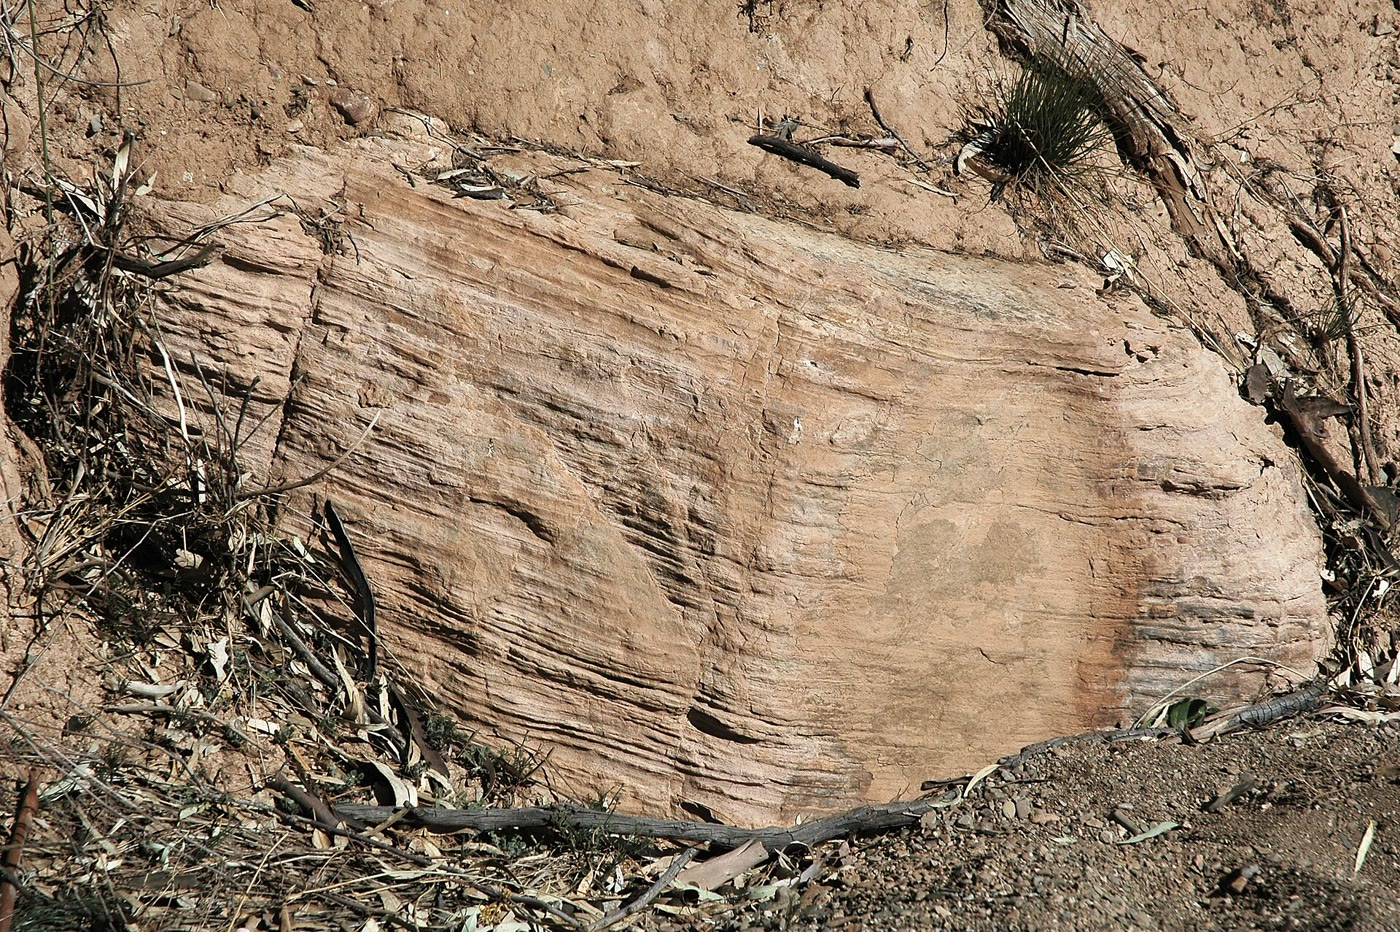
\includegraphics[width=0.66\linewidth]{images/book4/b2-18-cap-carbonate.jpg}
\par\smallskip{\small एक \omterm{def:b2:precambrian-earth:snowball}{टोपी कार्बोनेट}: नुक्कालीना संरचना का परतदार डोलोस्टोन,
फ़्लिंडर्स पर्वतमाला, दक्षिण ऑस्ट्रेलिया, जो मैरिनोअन हिमनदन के निक्षेपों पर टिका है
(परतें झुकी हुई हैं)। फ़ोटो: James St.~John, CC~BY~2.0 (Wikimedia Commons)।}
\end{omfigure}

क्रायोजेनियन की दो हिमगोल अवस्थाएँ अब ज्वालामुखीय राख के ज़िरकॉनों पर यूरेनियम--लेड आयु
और कार्बनिक-समृद्ध शेलों पर रीनियम--ऑस्मियम आयु से तिथि-निर्धारित हैं। स्टर्टियन 717.5 और
\qty{716.3}{Ma} के बीच शुरू हुआ और 659.3 और \qty{658.5}{Ma} के बीच समाप्त हुआ: \qty{58}{Myr} की बर्फ़,
आरंभ और अंत पूरे विश्व में समकालिक। मैरिनोअन 649.9 और
\qty{639.0}{Ma} के बीच शुरू हुआ, ढीले रूप से तिथि-निर्धारित, और 636.0 और \qty{634.7}{Ma} के बीच समाप्त हुआ: कम से कम
\qty{3}{Myr}। हर एक एकल \omterm{def:b2:precambrian-earth:snowball}{टोपी कार्बोनेट} के साथ समाप्त होता है, कभी कई के साथ नहीं। लौह संरचनाएँ,
जो एक अरब वर्ष से अनुपस्थित थीं, स्टर्टियन हिमनदीय निक्षेपों में लौटती हैं। कम से कम एक पहले की
हिमगोल अवस्था, साइडेरियन में लगभग \qty{2.4}{Ga} पर, GOE के समय आई; दोनों
प्रकरणों के बीच, कोई \qty{1.5}{Gyr} तक, लगभग कोई हिमचादर ज्ञात नहीं है।
% ledger: hoffman17:ages, hoffman17:cryochrons, hoffman17:cap, hoffman17:models, hoffman17:earlier

\begin{history}[एक विचित्र परिकल्पना से एक तिथि-निर्धारित सिद्धांत तक]
1964 में डब्ल्यू॰~बी॰ हारलैंड ने एक उत्तर प्रीकैम्ब्रियन हिमनदन के प्रमाणों की ओर ध्यान खींचा।
1968 और 1969 में एम॰~आई॰ बुदिको ने, और डब्ल्यू॰~डी॰ सेलर्स ने एक मिलते-जुलते प्रतिरूप से, पाया कि
\omterm{def:b2:precambrian-earth:ice-albedo}{हिम--एल्बिडो प्रतिपुष्टि} बर्फ़ के पर्याप्त आगे बढ़ने पर उसे भूमध्य रेखा तक फैला सकती है;
तब वैश्विक रूप से जमी पृथ्वी बिना वापसी की अवस्था लगती थी, और इसलिए ऐसी जो कभी हुई ही नहीं।
1981 में जे॰ वॉकर, पी॰ हेज़ और जे॰ कास्टिंग ने सिलिकेट अपक्षय के तापस्थापी का वर्णन किया और
देखा कि जमी पृथ्वी पर ज्वालामुखियों की कार्बन डाइऑक्साइड तब तक संचित होगी जब तक बर्फ़
न पिघले: अवस्था स्वयं को समाप्त कर सकती थी। 1992 में जे॰~एल॰ किर्शविंक ने प्रस्तावित किया कि यह वास्तव में
हुआ था, और उसे ``\omterm{def:b2:precambrian-earth:snowball}{हिमगोल पृथ्वी}'' नाम दिया; 1998 में पी॰~एफ़॰ हॉफ़मैन और सहयोगियों ने
``एक नियोप्रोटेरोज़ोइक \omterm{def:b2:precambrian-earth:snowball}{हिमगोल पृथ्वी}'' प्रकाशित किया, और सर्वहिमनदीय युगों को क्रायोक्रॉन कहा जाने लगा। 2004 से पहले
किसी क्रायोजेनियन हिमनदीय निक्षेप की रेडियोमितीय तिथि नहीं निकाली गई थी; ऊपर की तिथियाँ
उसके बाद के वर्षों का काम हैं।
\end{history}
% ledger: hoffman17:history

ज्वालामुखी बाहर निकलने का रास्ता हैं। बर्फ़ से ढकी पृथ्वी पर वर्षा और नदियाँ लगभग रुक जाती हैं, उनके साथ सिलिकेट
अपक्षय भी, और ज्वालामुखियों द्वारा मुक्त कार्बन डाइऑक्साइड वायु में तब तक संचित होती है
जब तक उसका ग्रीनहाउस बर्फ़ को पिघला न दे।

\begin{proposition}[कार्बन डाइऑक्साइड का संचय]\label{prop:b2:precambrian-earth:co2}
यदि कार्बन डाइऑक्साइड दर $F$ (प्रति वर्ष द्रव्यमान) से द्रव्यमान
$M_{\text{a}}$ और माध्य मोलर द्रव्यमान $\bar M$ वाले वायुमंडल में मुक्त होती है, बिना किसी अवशोषक के, तो उसके आयतन
मिश्रण-अनुपात को लगभग शून्य से $x$ तक लाने में लगने वाला समय है
\[
  \tau = \frac{x}{1 - x}\,\frac{M_{\mathrm{CO_2}}}{\bar M}\,\frac{M_{\text{a}}}{F} .
\]
\end{proposition}

\begin{proof}
वायुमंडल में अन्य गैसों के $n = M_{\text{a}}/\bar M$ मोल हैं। कार्बन डाइऑक्साइड के $n_c$ मोल जोड़ने पर
उसका मिश्रण-अनुपात $x = n_c/(n + n_c)$ होता है, अतः $n_c = n\,x/(1 - x)$, जिसका द्रव्यमान
$n_c M_{\mathrm{CO_2}}$ है; दर $F$ पर इसमें $\tau = n_c M_{\mathrm{CO_2}}/F$ लगता है।
\end{proof}

\begin{example}[बचने में कितना समय?]\label{ex:b2:precambrian-earth:escape}
आज के ज्वालामुखीय उत्सर्जन का उच्चतम वरीय अनुमान प्रति वर्ष \qty{0.26}{Gt} कार्बन
डाइऑक्साइड है। किसी क्रायोजेनियन हिमगोल को समाप्त करने के लिए आवश्यक
मिश्रण-अनुपात के अनुमान 0.01 से 0.1 तक हैं। $M_{\text{a}} =
\qty{5.1e18}{kg}$, $\bar M = \qty{28.97}{g.mol^{-1}}$ और $M_{\mathrm{CO_2}} =
\qty{44.01}{g.mol^{-1}}$ के साथ, $x = 0.01$ में $\frac{0.01}{0.99}\times1.519\times\qty{5.1e18}{kg}
/ \qty{0.26e12}{kg.yr^{-1}} = \qty{0.30}{Myr}$ लगते हैं, और $x = 0.1$ में \qty{3.3}{Myr}।
\end{example}
% ledger: usgs:volcanic-co2, hoffman17:co2, earth:Matm, earth:Mmol, ciaaw:abridged-2024
% values: co2_t001_Myr 0.301, co2_t01_Myr 3.311 (precambrian.py)

पूरी पृथ्वी पर \qty{1}{bar} भार वाले शुद्ध कार्बन डाइऑक्साइड के स्तंभ में उसी दर पर
\qty{20}{Myr} लगेंगे, वह आँकड़ा जो वॉकर, हेज़ और कास्टिंग ने दिया था। कुछ मिलियन वर्ष
लंबा समय है, पर स्टर्टियन \qty{58}{Myr} चला। या तो देहली ऊँची थी, या
उत्सर्जन कम, या जमी पृथ्वी में अब भी अवशोषक थे: युवा समुद्र-तल का अपक्षय,
जो बर्फ़ के नीचे नहीं रुकता, एक संभावित उम्मीदवार है। ऊर्जा-संतुलन प्रतिरूप में बचाव के लिए
हिमगोल की प्रभावी उत्सर्जकता को तब तक गिरना होगा जब तक उसका तापमान \qty{263}{K} तक न पहुँचे:
क्रायोजेनियन सूर्य के नीचे, जो आज का \qty{94}{\percent} था, 0.616 से 0.472 तक, यानी
कोई \qty{39}{W.m^{-2}} का अतिरिक्त रोधन (\cref{exo:b2:precambrian-earth:10})।
% ledger: hoffman17:co2, hoffman17:models, usgs:volcanic-co2
% values: one_bar_Myr 19.98, eps_melt_094 0.4716, forcing_melt_094 39.1 (precambrian.py)

जब अंततः भूमध्य रेखा पर बर्फ़ खुलती है, प्रतिपुष्टि उलटी चलती है: गहरा समुद्र अधिक
सूर्य-प्रकाश अवशोषित करता है, बर्फ़ पीछे हटती है, और प्रतिरूपों में हिम-रेखा लगभग
\qty{2}{kyr} में ध्रुवों की ओर दौड़ती है। तब पृथ्वी स्वयं को एक अंधेरी सतह पर विशाल ग्रीनहाउस के साथ पाती है, एक गर्म
परवर्ती अवस्था। उस जलवायु में बहुत तेज़ अपक्षय कैल्सियम, मैग्नीशियम और बाइकार्बोनेट को
समुद्र में उड़ेलता है, जहाँ \omterm{def:b2:precambrian-earth:snowball}{टोपी कार्बोनेट} अवक्षेपित होते हैं जबकि पिघला जल शेल्फ़ों को डुबोता है; कार्बन डाइऑक्साइड को
वापस नीचे लाने में कोई दस मिलियन वर्ष लगते हैं। हिमचादरें और \omterm{def:b2:precambrian-earth:snowball}{टोपी
कार्बोनेट}, लौह संरचनाएँ और समकालिक आयु वे कारण हैं जिनसे अधिकांश भूवैज्ञानिक अब स्वीकार करते हैं
कि क्रायोजेनियन हिमगोल अवस्थाएँ हुईं, यद्यपि वे कितनी कठोर थीं --- क्या भूमध्य रेखा पर खुले
जल की एक पट्टी बची रही, जैसा ``जल-पट्टी'' प्रतिरूप प्रस्तावित करते हैं --- इस पर अब भी बहस है।
% ledger: hoffman17:hysteresis, hoffman17:cap, hoffman17:debate

\section*{अभ्यास}\label{sec:b2:precambrian-earth:exercises}

अभ्यासों के आँकड़े, अन्यथा न कहा जाए तो: $\sigma = \qty{5.670e-8}{W.m^{-2}.K^{-4}}$;
$S_0 = \qty{1361}{W.m^{-2}}$; आज का एल्बिडो 0.294 और माध्य सतह-तापमान \qty{288}{K};
हिमगोल एल्बिडो 0.6; ढलान \qty{263}{K} से \qty{283}{K} तक; आज की प्रभावी उत्सर्जकता
0.616; गफ़ का नियम $L/L_0 = 1/(1 + 0.4\,t/t_\odot)$, वर्तमान से पहले के समय $t$ के लिए, $t_\odot =
\qty{4.567}{Gyr}$; \omterm{def:b2:precambrian-earth:greenstone}{कोमैटिआइट} लिक्विडस \qty{1616}{\celsius}, \qty{32.2}{\percent} MgO पर,
ढाल प्रति प्रतिशत \qty{18.0}{\celsius}; अर्धायु \ce{^{238}U} \qty{4.468}{Gyr}, \ce{^{235}U}
\qty{0.704}{Gyr}, \ce{^{232}Th} \qty{14.0}{Gyr}, \ce{^{40}K} \qty{1.248}{Gyr}।
% ledger: const:sigma, earth:TSI, earth:albedo, earth:Tsurf, hoffman17:models, gough81:luminosity, connelly12:cai, so16:liquidus, iaea:isotopes

\begin{exercise}[$\star$]\label{exo:b2:precambrian-earth:1}
(क) \omterm{def:b2:precambrian-earth:eons}{हेडियन}, \omterm{def:b2:precambrian-earth:eons}{आर्कियन} और \omterm{def:b2:precambrian-earth:eons}{प्रोटेरोज़ोइक} कितने समय तक चले? (ख) तीनों मिलकर पृथ्वी की आयु का
कितना अंश बनाते हैं? (ग) जब सबसे पुराना ज्ञात ज़िरकॉन क्रिस्टलित हुआ, और जब सबसे पुरानी चट्टानें बनीं,
तब पृथ्वी कितनी पुरानी थी?
\end{exercise}

\begin{exercise}[$\star$]\label{exo:b2:precambrian-earth:2}
आज बल्क सिलिकेट पृथ्वी प्रति किलोग्राम \ce{^{238}U} से \qty{1.917}{pW},
\ce{^{235}U} से \qty{0.082}{pW}, \ce{^{232}Th} से \qty{2.089}{pW} और
\ce{^{40}K} से \qty{0.818}{pW} मुक्त करती है ($\qty{1}{pW} = \qty{e-12}{W}$)। (क) \qty{3}{Gyr} पहले हर योगदान, और
कुल, निकालिए। (ख) तब से ऊष्मा-उत्पादन किस गुणक से गिरा है? (ग) कौन-सा समस्थानिक
आज अग्रणी है, और तब कौन-सा था?
\end{exercise}

\begin{exercise}[$\star$]\label{exo:b2:precambrian-earth:3}
\omterm{def:b2:precambrian-earth:greenstone}{कोमैटिआइट} तापमापी का उपयोग कीजिए। (क) \qty{28}{\percent} MgO वाले \omterm{def:b2:precambrian-earth:greenstone}{कोमैटिआइट} का
लिक्विडस क्या है? (ख) कौन-सी MgO मात्रा \qty{1500}{\celsius} के संगत है? (ग) स्पिनिफ़ेक्स बनावट वाले
किसी प्रवाह में संपूर्ण-शैल MgO \qty{38}{\percent} है। उसका लिक्विडस रेखा से क्यों नहीं
पढ़ा जाना चाहिए?
\end{exercise}

\begin{exercise}[$\star$]\label{exo:b2:precambrian-earth:4}
निम्नलिखित को क्रम में रखिए और उनकी अनुमानित आयु बताइए: \omterm{def:b2:precambrian-earth:goe}{महा ऑक्सीकरण घटना},
पहले स्ट्रोमैटोलाइट, मैरिनोअन हिमनदन का अंत, अंतिम सामान्य \omterm{def:b2:precambrian-earth:greenstone}{कोमैटिआइट},
सबसे पुरानी चट्टानें, ऑक्सीजन की दूसरी वृद्धि, पहले एडियाकरन जीवाश्म, पिलबारा की गुंबद-और-कील
संरचनाओं का अंत।
\end{exercise}

\begin{exercise}[$\star\star$]\label{exo:b2:precambrian-earth:5}
(क) जाँचिए कि आज की पृथ्वी की प्रभावी उत्सर्जकता 0.616 है। (ख) आज के सूर्य के नीचे हिमगोल
साम्य निकालिए। (ग) दिखाइए कि मध्य साम्य, \qty{275.5}{K}, $R = E$ को
\qty{0.5}{W.m^{-2}} के भीतर संतुष्ट करता है। (घ) वहाँ $R$ और $E$ के ढाल निकालिए, और निष्कर्ष निकालिए
कि वह अस्थायी है।
\end{exercise}

\begin{exercise}[$\star\star$]\label{exo:b2:precambrian-earth:6}
(क) गफ़ के नियम का उपयोग करके, \qty{2.4}{Ga} पहले और \qty{0.65}{Ga} पहले का सूर्य-प्रकाश आज के
अंशों के रूप में निकालिए। (ख) प्रतिरूप में, क्या आज की उत्सर्जकता के साथ हर तिथि पर गर्म जलवायु संभव है?
(ग) हॉफ़मैन और सहयोगी लिखते हैं कि साइडेरियन सूर्य क्रायोजेनियन सूर्य से लगभग \qty{10}{\percent} मंद
था। जाँचिए।
\end{exercise}

\begin{exercise}[$\star\star$]\label{exo:b2:precambrian-earth:7}
स्टर्टियन \qty{716.9}{Ma} से \qty{658.9}{Ma} तक चला (तिथि-निर्धारित अंतरालों के मध्य-बिंदु),
मैरिनोअन \qty{644.5}{Ma} से \qty{635.4}{Ma} तक। (क) उनकी अवधियाँ और उनके बीच का
अंतर्हिमनदीय काल निकालिए। (ख) इन आँकड़ों पर, क्रायोजेनियन काल, 720 से \qty{635}{Ma}, के कितने अंश में
बर्फ़ ने पृथ्वी को ढका? (ग) मैरिनोअन की अवधि केवल एक
मोटा आँकड़ा क्यों है?
\end{exercise}

\begin{exercise}[$\star\star$]\label{exo:b2:precambrian-earth:8}
(क) प्रति वर्ष \qty{0.26}{Gt} पर, बिना किसी अवशोषक के, ज्वालामुखियों को वायु को
0.05 के कार्बन डाइऑक्साइड मिश्रण-अनुपात तक लाने में कितना समय लगता है? (ख) यह 1750 के \qty{278}{ppm} का कितने गुना है? (ग) यदि उत्सर्जन का आधा समुद्र-तल
के अपक्षय द्वारा खप जाए, तो कितना समय लगेगा?
\end{exercise}
% ledger: usgs:volcanic-co2, earth:Matm, earth:Mmol, ciaaw:abridged-2024, ipcc:erf-2xco2

\begin{exercise}[$\star\star$]\label{exo:b2:precambrian-earth:9}
एक नियोप्रोटेरोज़ोइक डायमिक्टाइट में धारीदार पत्थर हैं, जिनमें से कुछ महीन परतदार पंक में पड़े हैं
जो उनके नीचे मुड़ा हुआ है। (क) यह मोड़ क्या बताता है? (ख) इसका पुराअक्षांश
\ang{10} है। हिमगोल परिकल्पना के लिए यह क्यों महत्त्वपूर्ण है? (ग) इसके ठीक ऊपर कुछ मीटर मोटा एक
गुलाबी परतदार डोलोस्टोन है। वह क्या है, और वह क्या अंकित करता है?
\end{exercise}

\begin{exercise}[$\star\star\star$]\label{exo:b2:precambrian-earth:10}
क्रायोजेनियन सूर्य के नीचे, $S = 0.94\,S_0$। (क) दिखाइए कि प्रतिरूप में गर्म अवस्था अब भी
मौजूद है, बमुश्किल, पर एक हिमगोल भी मौजूद है। (ख) आज की उत्सर्जकता के साथ हिमगोल का तापमान
निकालिए। (ग) वह उत्सर्जकता निकालिए जिस पर हिमगोल \qty{263}{K} तक पहुँचता है और
पिघलता है। (घ) उत्सर्जकता के परिवर्तन को \qty{263}{K} पर दीर्घ-तरंग विकिरण के अतिरिक्त रोधन में
बदलिए, \unit{W.m^{-2}} में।
\end{exercise}

\begin{exercise}[$\star\star\star$]\label{exo:b2:precambrian-earth:11}
(क) \cref{prop:b2:precambrian-earth:tipping} के क्रांतिक बिंदुओं का उपयोग करके दिखाइए कि
शैथिल्य-पाश की चौड़ाई, $S_{\text{m}}/S_{\text{f}}$, उत्सर्जकता पर निर्भर नहीं करती, और
उसे निकालिए। (ख) पाश को क्या सँकरा बनाएगा? (ग) कोई हिमगोल केवल उन
परिस्थितियों से दूर ही क्यों पिघल सकता है जिनमें वह जमा था?
\end{exercise}

\begin{exercise}[$\star\star\star$]\label{exo:b2:precambrian-earth:12}
गर्म साम्य के निकट ऊर्जा-संतुलन प्रतिरूप का समय-स्थिरांक, $\tau =
C/(E'(T^*) - R'(T^*))$, व्युत्पन्न कीजिए, और उसे \qty{50}{m} गहरी, घनत्व
\qty{1025}{kg.m^{-3}} और विशिष्ट ऊष्मा \qty{3992}{J.kg^{-1}.K^{-1}} वाली महासागरीय मिश्रित परत के लिए निकालिए। जब
सूर्य-प्रकाश बाएँ क्रांतिक बिंदु के निकट आता है, तब $\tau$ का क्या होता है, इस प्रतिरूप में और ऐसे प्रतिरूप में जिसका एल्बिडो
तापमान के साथ सुचारु रूप से बदलता है?
\end{exercise}
% ledger: noaa:seawater-1025, teos10:cp0

\begin{problem}[{सप्ताहांत समस्या --- एक अधिक गर्म युवा पृथ्वी}]\label{pb:b2:precambrian-earth:1}
यह समस्या युवा पृथ्वी का उसके भीतरी भाग से उसकी वायु तक अनुसरण करती है।
अभ्यासों के आँकड़े उपयोग कीजिए; बल्क सिलिकेट पृथ्वी में द्रव्यमान से \qty{0.0203}{ppm} यूरेनियम, \qty{0.0795}{ppm}
थोरियम और \qty{240}{ppm} पोटैशियम है, और उसके समस्थानिक प्रति किलोग्राम समस्थानिक \qty{95.13}{\micro W}
(\ce{^{238}U}), \qty{568.47}{\micro W} (\ce{^{235}U}), \qty{26.28}{\micro W} (\ce{^{232}Th}) और
\qty{28.47}{\micro W} (\ce{^{40}K}) मुक्त करते हैं। द्रव्यमान से, यूरेनियम
\qty{99.29}{\percent} \ce{^{238}U} और \qty{0.711}{\percent} \ce{^{235}U} है, और पोटैशियम
\qty{0.0120}{\percent} \ce{^{40}K}। तीन सार्थक अंकों तक पूर्णांकित कीजिए।

\noindent\textbf{भाग I --- भीतर से ऊष्मा।}
\begin{enumerate}
  \item आज बल्क सिलिकेट पृथ्वी के प्रति किलोग्राम हर समस्थानिक द्वारा मुक्त ऊष्मा निकालिए,
        \unit{pW.kg^{-1}} में।
  \item कुल निकालिए।
  \item हर समस्थानिक का क्षय-स्थिरांक निकालिए, \unit{Gyr^{-1}} में।
  \item \qty{2.7}{Gyr} पहले, जब पाइक हिल के \omterm{def:b2:precambrian-earth:greenstone}{कोमैटिआइट} उद्गारित हुए, हर योगदान निकालिए।
  \item तब का कुल, और आज के कुल से उसका अनुपात निकालिए।
  \item तब किस समस्थानिक ने सबसे अधिक ऊष्मा दी? आज वह इतनी कम क्यों देता है?
\end{enumerate}

\noindent\textbf{भाग II --- आर्कियन का सूर्य।}
\begin{enumerate}[resume]
  \item गफ़ के नियम से, \qty{2.7}{Ga} पहले का सूर्य-प्रकाश आज के अंश के रूप में, और
        \unit{W.m^{-2}} में, निकालिए।
  \item उस सूर्य-प्रकाश पर आज की उत्सर्जकता के साथ गर्म साम्य निकालिए। क्या वह प्रतिरूप की एक मान्य गर्म
        अवस्था है?
  \item उस सूर्य-प्रकाश पर हिमगोल साम्य निकालिए।
  \item गर्म एल्बिडो के साथ कौन-सी प्रभावी उत्सर्जकता पृथ्वी को \qty{288}{K} पर रखेगी?
  \item अकेली कार्बन डाइऑक्साइड 0.004 से \qty{0.03}{bar} के साथ यह कर सकती थी, \qty{2.5}{Ga} पर।
        लगभग \qty{1}{bar} के वायुमंडल में, यह 1750 के \qty{278}{ppm} का कितने गुना
        है?
  \item उस प्रक्रिया का नाम बताइए जिसने कार्बन डाइऑक्साइड को सैकड़ों मिलियन वर्षों तक ऐसे स्तर पर
        रखा।
\end{enumerate}

\noindent\textbf{भाग III --- एक हिमगोल और उसका अंत।}
\begin{enumerate}[resume]
  \item पहला हिमगोल, \qty{2.4}{Ga} पहले: तब का सूर्य-प्रकाश आज के अंश के रूप में निकालिए।
        क्या आज की उत्सर्जकता के साथ प्रतिरूप की गर्म अवस्था अब भी संभव है?
  \item प्रति वर्ष \qty{0.26}{Gt} कार्बन डाइऑक्साइड पर, 0.1 के मिश्रण-अनुपात तक पहुँचने में
        कितना समय लगता है?
  \item यदि मंदतर साइडेरियन सूर्य के नीचे देहली दुगुनी ऊँची, 0.2, थी, तो कितना समय?
  \item कौन-सी चट्टान हिमगोल के अंत को अंकित करती है, और कैसे?
  \item स्टर्टियन की लौह संरचनाओं को बर्फ़ के नीचे ऑक्सीजन-रहित महासागर की आवश्यकता क्यों है?
\end{enumerate}

\noindent\textbf{भाग IV --- कोमैटिआइट तापमापी।}
\begin{enumerate}[resume]
  \item दोनों प्रयोगों से \omterm{def:b2:precambrian-earth:greenstone}{कोमैटिआइट} रेखा का ढाल जाँचिए।
  \item पाइक हिल के एक \omterm{def:b2:precambrian-earth:greenstone}{कोमैटिआइट} द्रव में \qty{30}{\percent} MgO था। उसका लिक्विडस निकालिए।
  \item बारबर्टन \omterm{def:b2:precambrian-earth:greenstone}{कोमैटिआइट}, \qty{32.2}{\percent} MgO, का लिक्विडस निकालिए।
  \item \qty{12}{\percent} MgO वाले प्राथमिक कटक-बेसाल्ट का लिक्विडस निकालिए।
  \item इसके बजाय किलाउआ के ढाल, प्रति प्रतिशत \qty{20}{\celsius}, के साथ, बारबर्टन बिंदु से आरंभ करके,
        बेसाल्ट कितना गर्म होगा? ढाल के चयन से कितना अंतर पड़ता है?
  \item दोनों लावाओं के बीच तापमान का अंतर \omterm{def:b2:precambrian-earth:eons}{आर्कियन} और आज के प्रावार के बीच विभव तापमान के
        अंतर से अधिक क्यों है?
  \item सारांश में: सबसे गर्म \omterm{def:b2:precambrian-earth:eons}{आर्कियन} \omterm{def:b2:precambrian-earth:greenstone}{कोमैटिआइट} लावा आज के कटकों के किसी प्राथमिक बेसाल्ट से
        कितना अधिक गर्म था?
\end{enumerate}
\end{problem}
% ledger: ms95:pm-trace, dye:isotope-heat, iaea:isotopes, gough81:luminosity, cz20:archean-air, ipcc:erf-2xco2, usgs:volcanic-co2, hoffman17:co2, so16:liquidus, helz98:glass-thermometer, pierru22:komatiite
